\documentclass[11pt,a4paper]{ivoa}
\input tthdefs

\usepackage{array}
\newcolumntype{L}{>{\centering\arraybackslash}m{3cm}}

\title{VODML Mapping Lite Syntax}

% see ivoatexDoc for what group names to use here
\ivoagroup{DM}


\definecolor{gray}{rgb}{0.4,0.4,0.4}
\definecolor{darkblue}{rgb}{0.0,0.0,0.6}
\definecolor{maroon}{rgb}{0.5,0,0}
\definecolor{cyan}{rgb}{0.0,0.6,0.6}

\lstset{
  basicstyle=\ttfamily,
  columns=fullflexible,
  showstringspaces=false,
  commentstyle=\color{gray}\upshape
}

\lstdefinelanguage{XML}
{
  morestring=[b]",
  morestring=[s]{>}{<},
  morecomment=[s]{<?}{?>}, 
  morecomment=[s]{<!--}{-->},
  stringstyle=\color{black},
  identifierstyle=\color{darkblue},
  keywordstyle=\color{maroon},
  morekeywords={ref,utype,dmrole, dmtype, value}% list your attributes here
}
\author{François Bonnarel}
\author{Gilles Landais}
\author{Laurent Michel}
\author{Jesus Salgado}

\editor{Laurent Michel}

% \previousversion[????URL????]{????Concise Document Label????}
\previousversion{This is the first public release}
       

\begin{document}
\begin{abstract}
???? Abstract ????
\end{abstract}


\section*{Acknowledgments}

???? Or remove the section header ????

\section*{Conformance-related definitions}

The words ``MUST'', ``SHALL'', ``SHOULD'', ``MAY'', ``RECOMMENDED'', and
``OPTIONAL'' (in upper or lower case) used in this document are to be
interpreted as described in IETF standard RFC2119 \citep{std:RFC2119}.

The \emph{Virtual Observatory (VO)} is a
general term for a collection of federated resources that can be used
to conduct astronomical research, education, and outreach.
The \href{http://www.ivoa.net}{International
Virtual Observatory Alliance (IVOA)} is a global
collaboration of separately funded projects to develop standards and
infrastructure that enable VO applications.


\section{Introduction}

???? Write something ????

\lstset{language=XML}

\subsection{Role within the VO Architecture}

\begin{figure}
\centering

% As of ivoatex 1.2, the architecture diagram is generated by ivoatex in
% SVG; copy ivoatex/archdiag-full.xml to archdiag.xml and throw out
% all lines not relevant to your standard.
% Notes don't generally need this.  If you don't copy archdiag.xml,
% you must remove archdiag.svg from FIGURES in the Makefile.

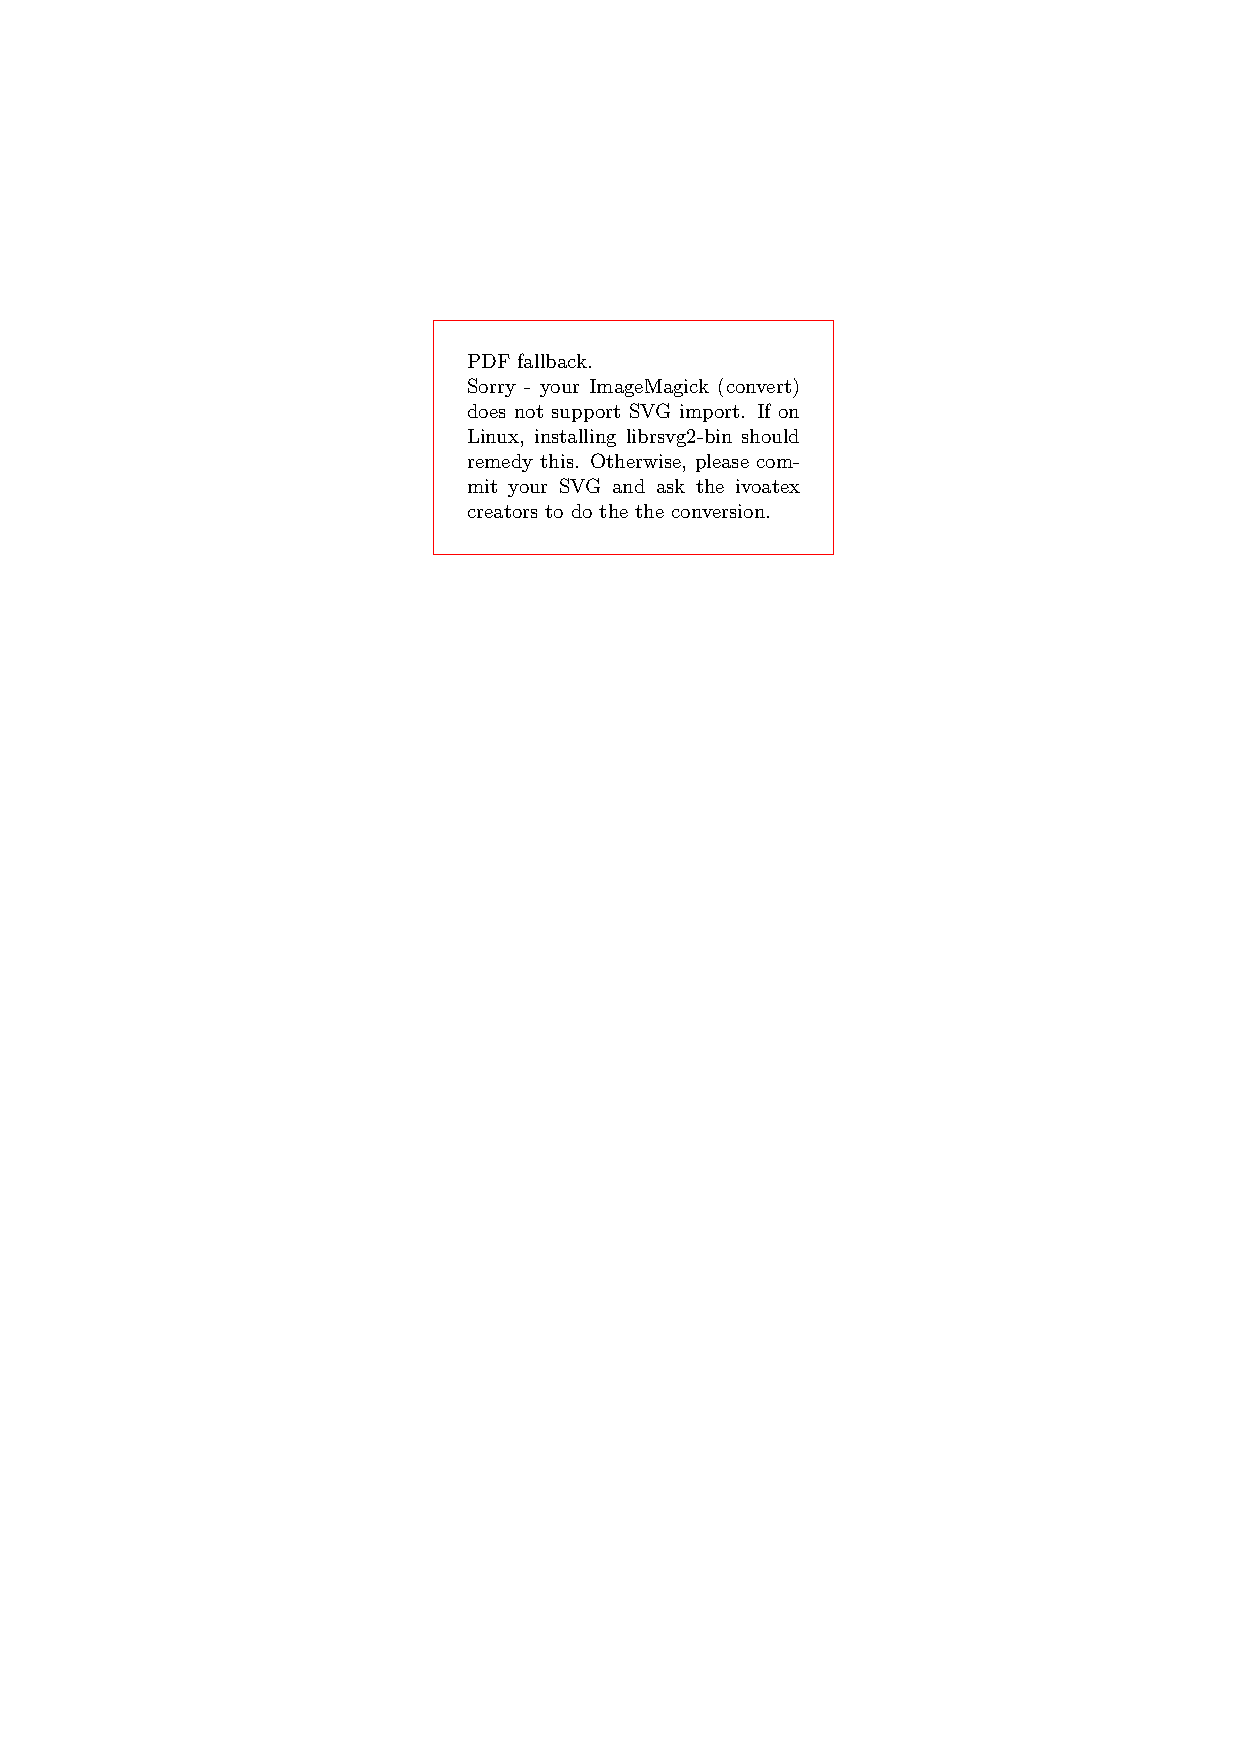
\includegraphics[width=0.9\textwidth]{role_diagram.pdf}
\caption{Architecture diagram for this document}
\label{fig:archdiag}
\end{figure}

Fig.~\ref{fig:archdiag} shows the role this document plays within the
IVOA architecture \citep{note:VOARCH}.

???? and so on, LaTeX as you know and love it. ????

\section{Use Cases and Requirement}

This alternative mapping syntax keeps the same basics as the original proposal:

\section{Syntax}

\begin{itemize}
	\item This mapping syntax support directive for the clients which are not part of the model (e.g. aggregation request or data filters).
	\item The mapping as an explicit entry point, telling to the client what is the VOTable content.
	\item Processing this alternate syntax require for the client to apply rules not states in the VOTable itself.
\end{itemize}

\begin{itemize}
    \item The mapping is located in a \texttt{<VODML>} block, child of \texttt{<VOTABLE>}.
    \item The mapping elements reflect the model structure.
    \item The \texttt{<VODML>} block starts with a list of implemented models.
    \item There is one \texttt{<TEMPLATES>} per mapped \texttt{<TABLE>}.
    \item There is one \texttt{<GLOBALS>} block containing data shared by the whole mapping.
\end{itemize}

\subsection{GLOBALS}

Contains  \texttt{INSTANCE}s with fixed values that can be used everywhere in the \texttt{VODML}.


\begin{lstlisting}[caption={INSTANCE bloc example},captionpos=b]
  <GLOBALS>
    <INSTANCE ID="SpaceCoordFrame" dmrole="">
      <INSTANCE dmrole="coords:SpaceFrame.refPosition" dmtype="coords:StdRefLocation">
        <VALUE dmrole="coords:StdRefLocation.position" dmtype="ivoa:string" value="NoSet"/>
      </INSTANCE>
      <VALUE dmrole="coords:SpaceFrame.spaceRefFrame" dmtype="ivoa:string" value="ICRS"/>
      <VALUE dmrole="coords:SpaceFrame.equinox" dmtype="coords:Epoch" value="NoSet"/>
    </INSTANCE>
    <INSTANCE >
      ... 
    </INSTANCE>
    ...
  </GLOBALS>
\end{lstlisting}




\begin{table}[ht!]
     \begin{tabular}{|p{3cm}|p{7cm}|}
       \hline Child &  Role\\
       \hline  \texttt{INSTANCE}    &  \texttt{GLOBALS} children must be \texttt{INSTANCE} . \\       
       \hline 
     \end{tabular}
     \caption{Supported  \texttt{GLOBALS} children} 
 \end{table}

 \texttt{GLOBALS} has no attributes. 


\subsection{INSTANCE}

Mapping for either object type or a datatype instances.


\begin{lstlisting}[caption={INSTANCE bloc example},captionpos=b]
<INSTANCE dmrole="ds:dataset.Dataset.dataID" dmtype="ds:dataset.DataID" ID="_ds_">
    <VALUE dmrole="ds:dataset.DataID.title" value="Gaia TS Mapping Test" />
    <VALUE dmrole="ds:dataset.DataID.datasetID" value="ivoa://gaia/ts/12345" />
    <VALUE dmrole="ds:dataset.DataID.creatorDID" value="ivoa://esa/gaia/" />
    <VALUE dmrole="ds:dataset.DataID.version" value="0.0" />
    <VALUE dmrole="ds:dataset.DataID.date" value="2018:11:11" />
    <VALUE dmrole="ds:dataset.DataID.creationType" value="LiteMappingTest" />
    <INSTANCE dmrole="ds:dataset.DataID.creator" dmtype="ds:dataset.Creator">
        <INSTANCE dmrole="ds:party.Role.party" dmtype="ds:party.Individual">
            <VALUE dmrole="ds:party.Party.name" value="VODML-Team" />
       </INSTANCE>
    </INSTANCE>
</INSTANCE>
\end{lstlisting}




\begin{table}[ht!]
     \begin{tabular}{|p{3cm}|p{7cm}|}
       \hline Child &  Role\\
       \hline  \texttt{INSTANCE}    & Another embedded instance . \\       
       \hline  \texttt{VALUE}    & Primitive attribute . \\       
       \hline  \texttt{COMPOSITION}    & Composition with a limited set of  \texttt{INSTANCE} e.g. author list\\      
       \hline  \texttt{ARRAY}    & Composition with a set of  \texttt{INSTANCE} corresponding each to one row of the data table. \\
       \hline  \texttt{FILTER}    & TbC \\
       \hline 
     \end{tabular}
     \caption{Supported  \texttt{INSTANCE} children} 
 \end{table}

\begin{table}[ht!]
     \begin{tabular}{|p{1.5cm}|p{4cm}|p{7cm}|}
       \hline Attribute & Requ. level & Role\\
       \hline  @dmrole   & Mandatory & VODML role of the instance. May be empty for instances child of 
                                      \texttt{GLOBALS}  \\
       \hline  @dmtype  & Mandatory except for reference & VODML type of the instance.   \\
       \hline  @dmref  & Mandatory for reference & reference to another instance in the mapping bloc. \\          
       \hline  @ID  & Mandatory if the instance is referenced by other instances & Unique identifier of the instance. \\
       \hline 
     \end{tabular}
     \caption{Supported attributes for  \texttt{INSTANCE}} 
 \end{table}

\begin{table}[ht!]
\begin{tabular}{|p{1.5cm}|p{1.5cm}|p{1.5cm}|p{5cm}|}
\hline @dmrole & @dmref &  @dmtype &  use case\\
\hline  yes & yes &  & Reference to another instance. The element must have no child  \\
\hline  yes &  & yes  & Instance serialization The element must enclose the instance content  \\
\hline 
\end{tabular}
     \caption{Supported attribute patterns for  \texttt{INSTANCE}} 
 \end{table}

\subsection{VALUE}

Mapping for primitive attributes. \texttt{VALUE}  are the model leaves that point onto real data. 


\begin{lstlisting}[caption={VALUE examples},captionpos=b]
<INSTANCE dmrole="model:value.example" dmtype="model:value.Example">
    <VALUE dmrole="model:preset.value" value="Preset Value" />    
    <VALUE dmrole="model:ref.value" ref="fieldID" />    
    <VALUE dmrole="model:reforpreset.value" value="Preset Value" ref="fieldID" />
 </INSTANCE>
\end{lstlisting}

 \texttt{VALUE}s have no children. 

\begin{table}[ht!]
     \begin{tabular}{|p{1.5cm}|p{4cm}|p{7cm}|}
       \hline Attribute & Requ. level & Role\\
       \hline  
      @dmrole   & MUST & VODML role of the instance attribute.\\       
       \hline 
      @dmtype   & MUST & VODML type of the instance attribute.\\
       \hline  
      @value  & MUST if no \texttt{@ref } element attribute. \newline MAY if \texttt{@ref} element attribute 
                    & Value of the instance attribute. 
                     \newline If  \texttt{VALUE} has also a \texttt{@ref}, \texttt{@ref} MUST be resolved first.
                     \texttt{VALUE}  MUST be taken when \texttt{@ref} cannot be resolved \\
        \hline
       @ref  & MUST if no \texttt{@value} element attribute. 
                     \newline MAY if \texttt{@value} element attribute 
                & Reference of the data element (\texttt{FIELD} or \texttt{PARAM}).  
                    \newline MUST refer to an element of the \texttt{TABLE}  referenced by the current     
                    \texttt{TEMPLATE}                    
                    \newline The client MUST first look for a \texttt{FIELD} matching \texttt{@ref}. 
                    \newline In case of failure, it MUST look for a \texttt{PARAM}
                    \\
       \hline 
     \end{tabular}
     \caption{Supported attributes for  \texttt{VALUE}} 
 \end{table}

\begin{table}[ht!]
  \begin{tabular}{|p{1.5cm}|p{1.5cm}|p{1.5cm}|p{1.5cm}|p{5cm}|}
    \hline @dmrole  &  @dmtype &  @ref &  @value &  Role\\
    \hline  yes & yes &  yes & & The instance attribute must take the value pointed by \texttt{@ref} \\
    \hline  yes & yes &  & yes & The instance attribute must take the value set in  \texttt{@value} \\
    \hline  yes & yes &  yes & yes 
              & The instance attribute must take the value pointed by \texttt{@ref} 
                  \newline and the this set in  \texttt{@value} if \texttt{@ref} cannot be resolved\\
    \hline 
  \end{tabular}
  \caption{Supported attribute patterns for  \texttt{VALUE}} 
 \end{table}

\appendix
\section{Changes from Previous Versions}

No previous versions yet.  
% these would be subsections "Changes from v. WD-..."
% Use itemize environments.


% NOTE: IVOA recommendations must be cited from docrepo rather than ivoabib
% (REC entries there are for legacy documents only)
\bibliography{ivoatex/ivoabib,ivoatex/docrepo}


\end{document}
